\documentclass[tikz, border = 5pt]{standalone}

\begin{document}
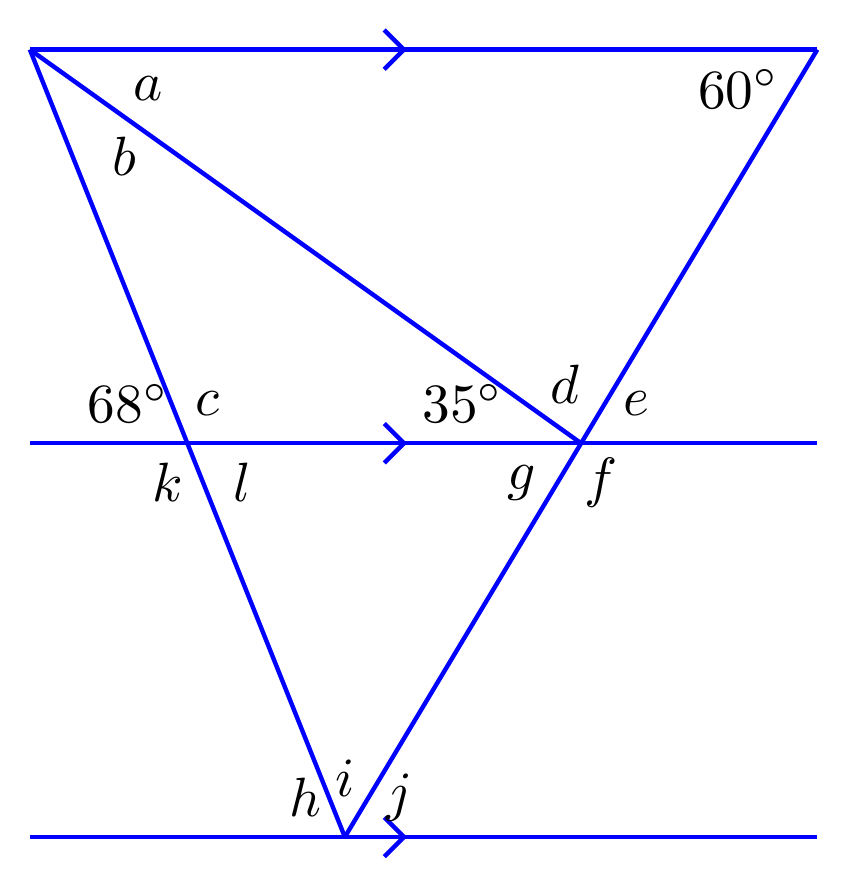
\begin{tikzpicture}

% grid
%\draw[help lines, step = 1cm] (0, 0) grid (10, 12);

\draw[ultra thick, smooth,blue, -] (0,11) -- (10,11);
\draw[ultra thick, smooth,blue, -] (0,11) -- (7,6);
\draw[ultra thick, smooth,blue, -] (10,11) -- (4,1);
\draw[ultra thick, smooth,blue, -] (0,11) -- (4,1);
\draw[ultra thick, smooth,blue, -] (0,6) -- (10,6);
\draw[ultra thick, smooth,blue, -] (0,1) -- (10,1);

% Arrows
\draw[ultra thick, smooth,blue, -] (4.5,11.25) -- (4.75,11);
\draw[ultra thick, smooth,blue, -] (4.5,10.75) -- (4.75,11);
\draw[ultra thick, smooth,blue, -] (4.5,6.25) -- (4.75,6);
\draw[ultra thick, smooth,blue, -] (4.5,5.75) -- (4.75,6);
\draw[ultra thick, smooth,blue, -] (4.5,1.25) -- (4.75,1);
\draw[ultra thick, smooth,blue, -] (4.5,0.75) -- (4.75,1);

% labels
\node[scale=2] at (1.5,10.5) {$a$};
\node[scale=2] at (1.2,9.65) {$b$};
\node[scale=2] at (2.25,6.5) {$c$};
\node[scale=2] at (6.8,6.75) {$d$};
\node[scale=2] at (7.7,6.5) {$e$};
\node[scale=2] at (7.25,5.5) {$f$};
\node[scale=2] at (6.25,5.5) {$g$};
\node[scale=2] at (3.5,1.5) {$h$};
\node[scale=2] at (4,1.75) {$i$};
\node[scale=2] at (4.7,1.5) {$j$};
\node[scale=2] at (1.75,5.5) {$k$};
\node[scale=2] at (2.7,5.5) {$l$};
\node[scale=2] at (5.5,6.5) {$35^{\circ}$};
\node[scale=2] at (9,10.5) {$60^{\circ}$};
\node[scale=2] at (1.25,6.5) {$68^{\circ}$};

\end{tikzpicture}
\end{document}
